\newacronym{DPA}{DPA}{Dinamic programming algorithm}

We will define the pairwise alignment problem \cite{Srivastava2016} to deal with
the registration problem of two functions using a global criterion.

Let $f_1, f_2 \in \mathcal{F}$ be functional observations of a general space
$\mathcal{F}$ and $E: \mathcal{F} \times \mathcal{F} \rightarrow \mathbb{R}^+$ an energy
functional. The alignment problem may be understood as the search of a warping
function $\gamma^*$ which minimizes the energy between the two functions, i.e.,

\begin{equation}[EQ:ENERGY]{Creterion for pairwise alignment}
\gamma^* = \underset{\gamma \in \Gamma}{ \operatorname{argmin}} \, E[f_1, f_2 \circ \gamma].
\end{equation}

When a warping $\gamma^*$ fulfills this property, we will say that $f_1$ is
registered to $f_2 \circ \gamma^*$. In the Figure \ref{SBFIG:PAIRWISE1} it is
shown an example where two functions have been registered using this approach.

\begin{figure}[Pairwise alignment]{FIG:PAIRWISE}{Pairwise alignment}
	\subfigure[SBFIG:PAIRWISE1]{Alignment of $f_1$ to $f_2$}{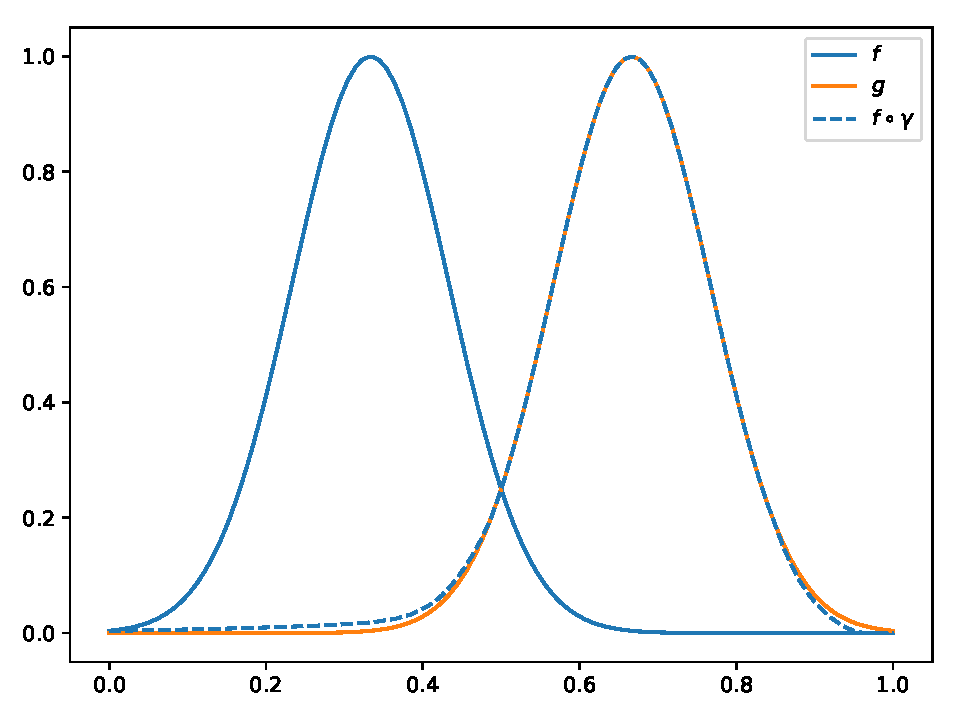
\includegraphics[width=7.5cm]{pairwise-alignment}} \quad
	\subfigure[SBFIG:PAIRWISE2]{Warping built by the DPA algorithm}{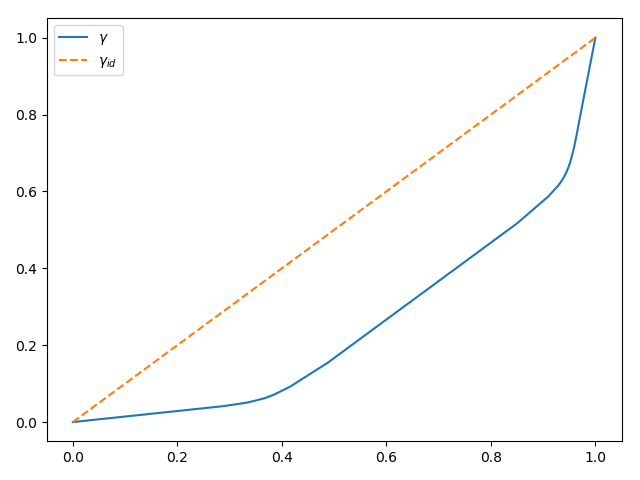
\includegraphics[width=7.5cm]{pairwise-alignment-warping}}
\end{figure}

To estimate $\gamma^*$, we will explore different paths that the
reparameterization may take in a discretized grid, trying to minimize the energy
term. This algorithm, described in deatil in \cite{Srivastava2016}, is called \ac{DPA},
because it makes use of dynamic programming techniques to search the optimal
path \cite{dpa}.

Given a set of functions $\{f_i\}_{i=1}^n \subset \mathcal{F}$, the
groupwise alignment problem will consist in the search of warping functions
$\{\gamma_i^* \}_{i=1}^n \subset \Gamma$ to align each of the functions with the
rest of them. To achieve this, we will build a target function $\mu$, also
called template, to which all the curves will be aligned. For instance,
the cross-sectional mean of the functions can be used as target, which is
the average function $\frac{1}{n}\sum_{i=1}^{n}f_i$.

A possible choice for the energy term would be to take
$E[f-1,f_2]= \|f-1 - f_2\|_{\mathbb{L}^2}^2=\int_\mathcal{F} (f_1 - f_2)^2$.
This criterion is not commonly used in practice because three
problems will arise that will not make it adequate: the pinching effect, the
lack of symmetry and the inverse inconsistency \cite{Marron2015}.
In what follows we provide a a short description of these issues.
